\section{Experimental Results}
\label{sec:expresults}
This section presents experimental results obtained applying Euclidean and Riemannian distances in SSVEP classification task. 
%The performances are compared with LDA. 
The first part of this section describes the data used and the second part provides the assessment of the classification for the considered distances and divergences. %classifications accuracies obtained. 

\subsection{SSVEP Dataset}
The experimental study is conducted on multichannel EEG signals recorded during an SSVEP-based BCI experiment~\cite{kalunga_hybrid_2014}.   
EEG are recorded on $\dc=$ 8 channels from 12 subjects.
The subjects are presented with $\dF=$ 3 visual target stimuli blinking respectively at 13Hz, 21Hz and 17Hz. %$\text{freq}=$
It is a $\dK=$ 4 classes setup combining $\dF=$ 3 stimulus classes and one resting class (no-SSVEP).
In a session, 32 trials are recorded: 8 for each visual stimulus and 8 for the resting class. 
A trial is 4 second long. 
The number of sessions recorded per subject varies from 2 to 5.
For each subject, a test set is made of 32 trials while the remaining trials (which might vary from 32 to 128) make up for the training set.
\begin{figure}[h!]
\centering
\subfigure[]{
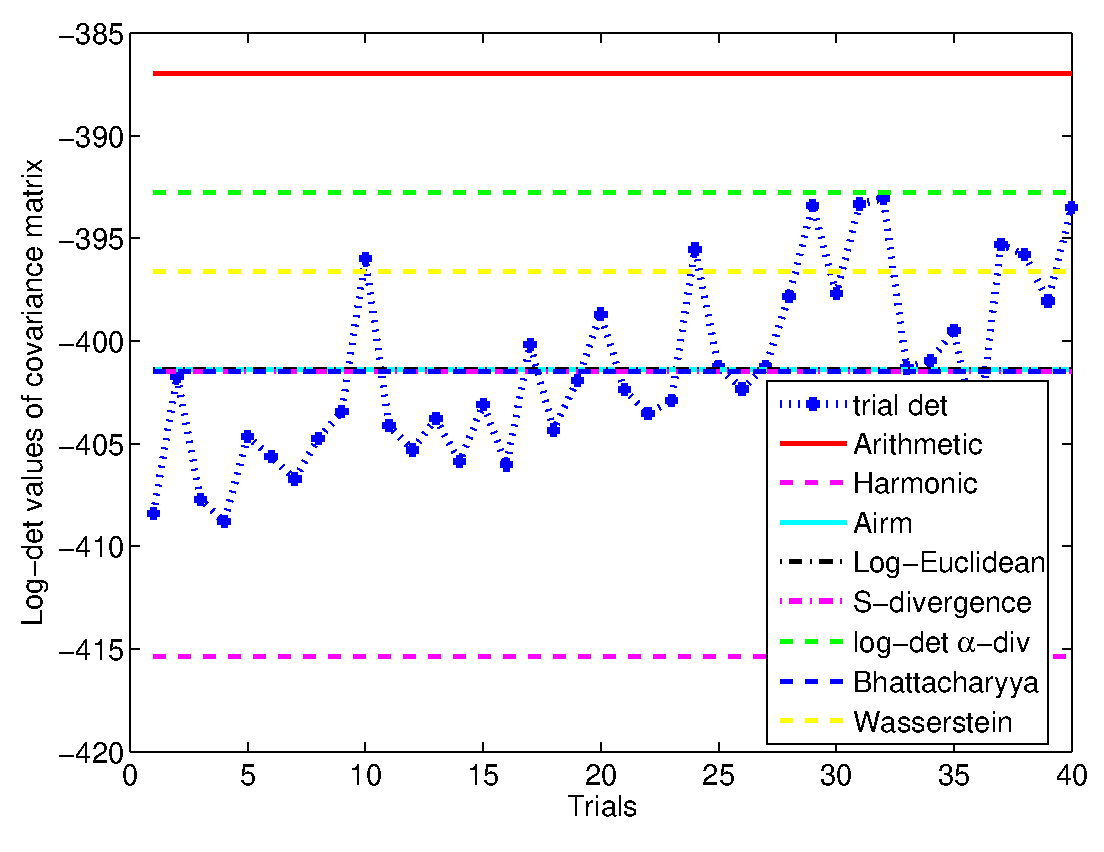
\includegraphics[width=0.46\textwidth]{Figures/swel.eps}
\label{fig:swel}
}
\subfigure[]{
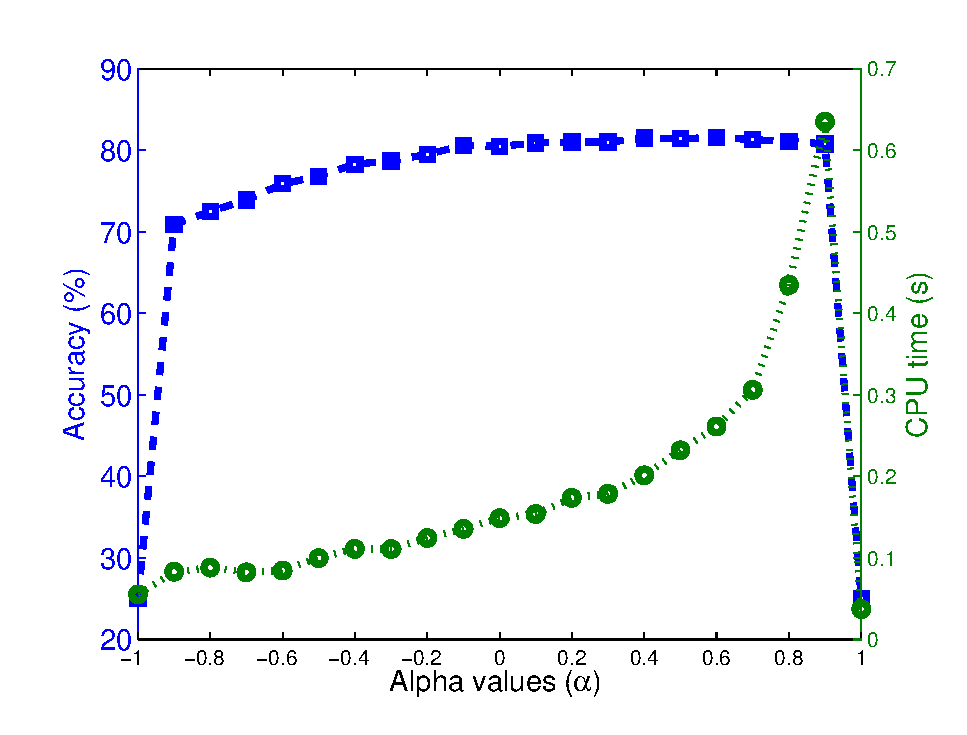
\includegraphics[width=0.49\textwidth]{Figures/alpha_cross.eps}
\label{fig:alphacross}
}
\caption{(a): Swelling effect of Arithmetic mean shown through log-determinant values. Training trials are taken from the 13Hz class of the subject with the highest BCI performance. Log-determinant values are given for each trial covariance (points), and for means of Table~\ref{tab:dist} (horizontal lines). (b): Classification accuracy and CPU time, obtained with $\alpha$-divergence for $-1\leqslant \alpha  \leqslant 1$.} 
\label{fig:swel_alpha}
\end{figure} 

\subsection{Results and Discussion}

\iflatexml\else \changes{ \fi
Discuss the invariance to right- and left-multiplication by positive matrices. It brings a significant advantage over Euclidean metrics, in terms of electrode placement and unforseen displacement in electrodes position, and can even alleviate anatomical differences.
\iflatexml\else } \fi
%\begin{figure}[h!]
%\centering
%\subfigure[]{
%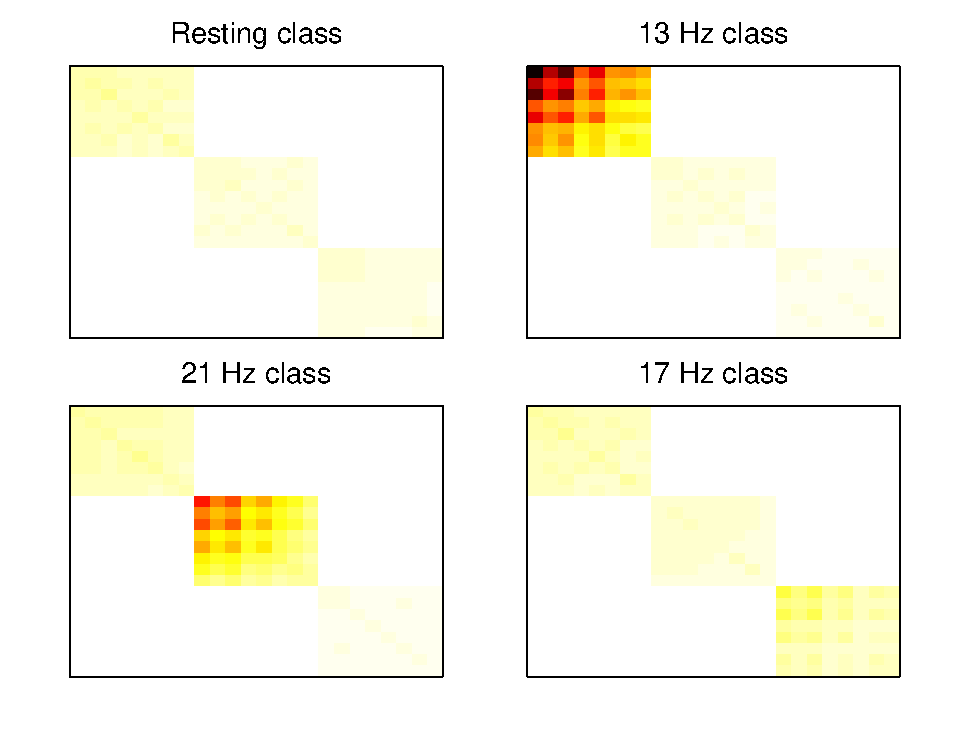
\includegraphics[width=0.47\textwidth]{Figures/covmat.eps}
%\label{fig:covmat12}}
%\subfigure[]{
%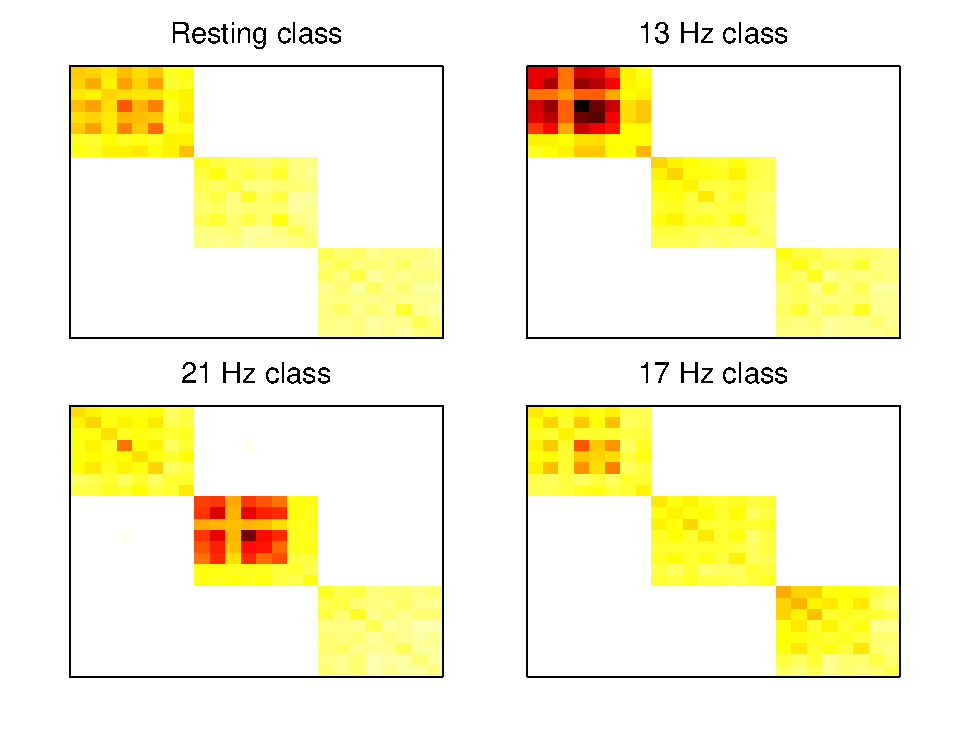
\includegraphics[width=0.47\textwidth]{Figures/covmat11.eps}
%\label{fig:covmat11}}
%\caption{Representation of covariance matrices: each image is the covariance matrix mean $\Pm^{(\ci)}$ of the class $\ci$, for one session of the recording. The diagonal blocks show the covariance in different frequency bands, i.e. 13Hz in the upper-left block, 21Hz in the middle, and 17Hz in the bottom-right. Subjects with highest (a) and lowest (b) BCI performance.}
%\label{fig:covmat}
%\end{figure}

